
As robotic applications flourish in our modern world, there is an increasing need for  high reduction, high torque, and low backlash actuator systems. These actuators are present in all types of robotic equipment. This need is true in space flight applications as well. A notable recent example includes the Curiosity rover from NASA's Jet Propulsion Laboratory \cite{curiosity} that uses primarily Harmonic Drives. Currently, Harmonic Drives are the primary reduction method when high ratio and compact design are required. These reducers come in limited reduction ratio options, and can grown quite heavy to withstand the high torque applications. This leads to the need for an alternative high reduction, compact drive system for these applications. 

\subsection{Cycloidal Drive Motivation}

Cycloidal drives are potentially an apt replacement for these Harmonic Drives as they can offer large a large reduction in a small package. They provide some distinct advantages as well in situations where small backlash is acceptable, such as their ability to be customized into the system directly and are made of relatively easy to manufacture parts, unlike a Harmonic Drive. In addition, the torque to weight ratio typically higher for cycloidal drives of this style, the cycloid presented in this work is X (TODO) kg and a comparable Harmonic Drive is 19.8kg.
However, there is insufficient data available for the true efficiency and characteristics of these drives. The primary contribution of this research shows the efficiency of a cycloidal drive system designed for a robotic application. This is done through an extended drive cycle test for burn-in to steady state performance over 37K (TODO) revolutions through 80 (TODO) hours and efficiency testing over the torque and speed range of this system. 

   \begin{figure}[!b]
      \centering
      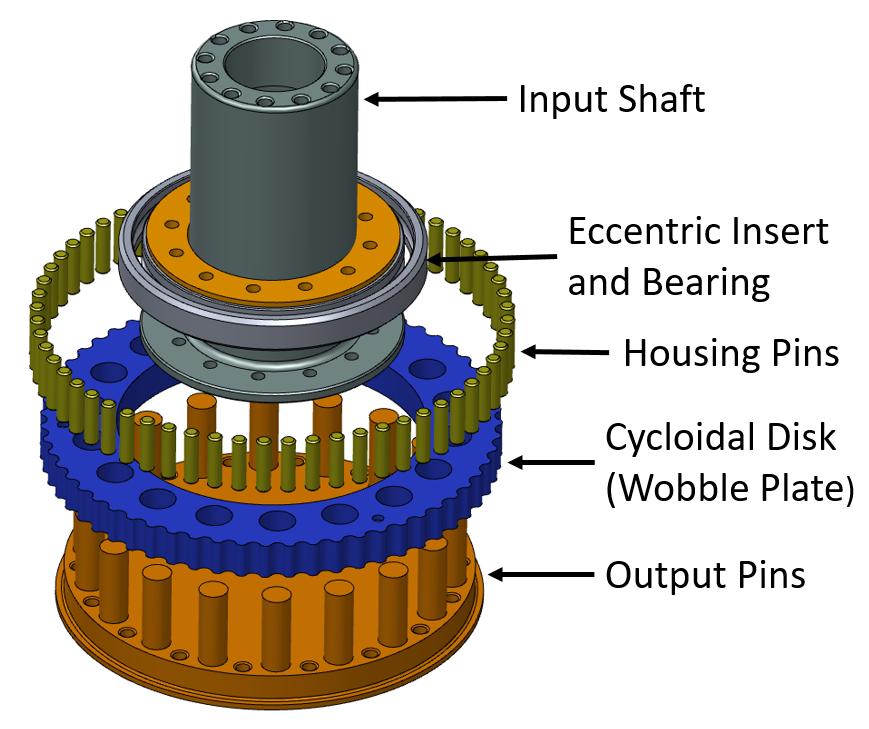
\includegraphics[width=0.50\linewidth]{cycloid_cartoon_v2}
      \caption{Simple rendering of the key elements that create a cycloidal drive. A drive shaft spins a cycloidal disk (wobble plate) via an eccentric circle. The wobble plate reacts against the housing pins to create a counter-rotation, harnessed by the output pins.}
      \label{cycloid_cartoon}
   \end{figure}
   
\subsection{Cycloidal Drive Background}
Cycloidal drives were proposed as early as 1956 by Botsiber and Kingston \cite{1956}. The premise of this design leverages a plate, referred to as the wobble plate, with lobes interacting with pins in the housing designed using trochoidal motion being spun on an eccentric shaft with a bearing. This induces a counter-clockwise motion of the plate and this is harnessed with the interior pins as the output of the mechanism. This basic layout can be seen in Fig \ref{cycloid_cartoon}. This geartrain design has been used in industry for high torque, high shock load applications for many years\footnote{http://www.nabtescomotioncontrol.com/engineering.php}. However, in many of these applications, all of the interacting surfaces like the housing pins and output pins use needle roller bearings to transmit load. This allows for higher efficiency and load carrying capability but it also increases mass and size for a given design need. In the robotic industry, groups are striving to reduce the mass and size of these actuators while still achieving the high reduction and load capabilities. The primary method to do this is to eliminate many of the rolling elements at the interaction points between the wobble plate, housing pins, and output pins. This allows for very compact and strong designs to be considered but leaves the potential for larger losses and lower system lifetime. 

Many works have been presented on the subject of the theoretical design of these cycloidal drives \cite{on_the_lobe} \cite{hwang_hsieh}, designing with machine tolerances \cite{design_and_application}, contact and stress analysis \cite{li}, and performance characteristics such as torque ripple and backlash \cite{hsieh_traditional} \cite{hsieh_dynamics}. Please see See Section \ref{design} for details. These works lay a solid foundation to a designer with the equations and design considerations to take while designing a cycloid. However, there has been very little work done in the area of in-use characteristics aside from the theoretical calculations and models. 

Many of researchers have explored and presented calculations for the efficiency, Malhorta and Parameswaran calculated between 98\% and 88\% efficiency for designs \cite{Malhorta} and Sensinger predicted 95\% \cite{unified_approach}. Later, Sensinger and Lipsey performed a short one and a half hour study on the efficiency of a cycloid test article \cite{cycloid_vs_harmonic} showing efficiencies in the 40\% range for fused roller designs, and 60\% for pin designs. Fused rollers designs machine the roller designs manufacture the ring pins are part of the housing, pin roller designs insert pins into holes to allow relative motion during contact. In addition, Hsieh verified the stress present in the drives in simulation and in use and demonstrated lower stress levels and torque ripple when using fused rollers \cite{hsieh_dynamics}. 

The aim of this work is to utilize a custom cycloid design for a NASA rover application and show the in-use efficiency characteristics over a more extended duration test. First, the authors will detail the actuator design in Section \ref{design}. Second, a description of the experimental setup and procedure is provided in Section \ref{methods}. Finally, the results and analysis of this high torque actuator and its implications are presented and discussed in Section \ref{results} and Section \ref{discussion}. 